\subsection{Problem Statement}

Consider an EPC contractor managing a portfolio $\mathcal{P} = \{1, 2, \ldots, N\}$ of $N$ projects over a planning horizon $T$. Each project $i \in \mathcal{P}$ is characterized by:

\begin{itemize}
    \item Budget at Completion (BAC): $\text{BAC}_i \in \R^+$
    \item Planned duration: $D_i \in \N^+$ periods
    \item Start time: $t_i^{\text{start}} \in \{0, 1, \ldots, T\}$
    \item Profit margin: $\pi_i \in [0, 1]$
    \item Total contract revenue: $R_i = \text{BAC}_i \times (1 + \pi_i)$
\end{itemize}

At each decision epoch $t \in \{0, 1, \ldots, T-1\}$, the contractor must allocate budget across active projects subject to a total budget constraint $B_t$. The allocation decision affects project progress, which in turn determines future cashflow requirements and revenue collection through milestone-based payments.

The fundamental challenge arises from \textit{contractor performance uncertainty}: the actual spending rate and progress of each project deviate stochastically from planned values due to execution risks (labor productivity, material delays, design changes, weather, etc.). This uncertainty creates unknown state transition probabilities, making classical optimization methods inadequate.

\subsection{Rolling Horizon Framework}

To handle variable-duration portfolios (12--60 months) while maintaining computational tractability, we adopt a \textit{rolling horizon} architecture with fixed planning window $H = 12$ periods (months). At each timestep $t$, the decision-maker:

\begin{enumerate}
    \item Observes current portfolio state $s_t$
    \item Solves a finite-horizon problem over $[t, t+H-1]$
    \item Executes only the first-period action $a_t$
    \item Advances to $t+1$, observes new state $s_{t+1}$, and re-plans
\end{enumerate}

This framework offers three key advantages:

\textbf{(1) Bounded state space:} The RL agent trains on fixed $H$-period episodes, preventing state-space explosion for long portfolios.

\textbf{(2) Adaptive re-planning:} New information (performance updates, budget changes) is incorporated at each re-planning step, enabling dynamic adjustment.

\textbf{(3) Real-world alignment:} The 12-month horizon matches industry practice (annual budget cycles with quarterly/monthly reviews).

\begin{figure}[h]
\centering
\resizebox{0.9\columnwidth}{!}{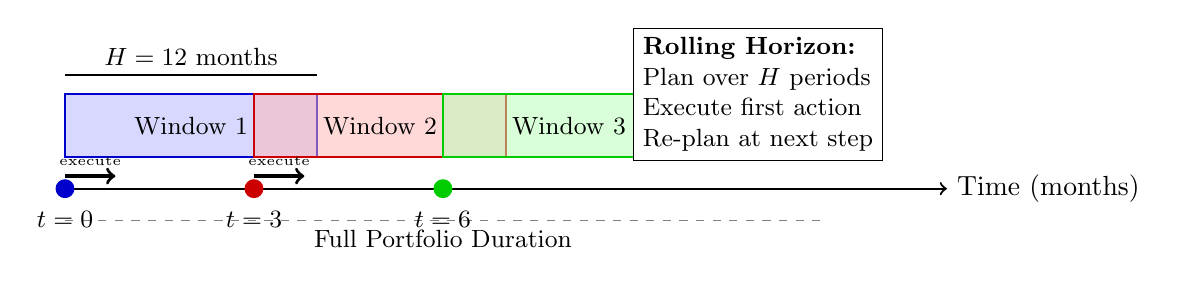
\begin{tikzpicture}[scale=0.8]
    % Timeline
    \draw[thick, ->] (0,0) -- (14,0) node[right] {Time (months)};
    
    % Full horizon indicator
    \draw[dashed, gray] (0,-0.5) -- (12,-0.5);
    \node[below] at (6,-0.5) {\small Full Portfolio Duration};
    
    % Rolling windows
    % Window 1
    \fill[blue!30, opacity=0.5] (0,0.5) rectangle (4,1.5);
    \draw[thick, blue!80!black] (0,0.5) rectangle (4,1.5);
    \node at (2,1) {\small Window 1};
    \fill[blue!80!black] (0,0) circle (0.15);
    \node[below] at (0,-0.2) {\small $t=0$};
    
    % Window 2
    \fill[red!30, opacity=0.5] (3,0.5) rectangle (7,1.5);
    \draw[thick, red!80!black] (3,0.5) rectangle (7,1.5);
    \node at (5,1) {\small Window 2};
    \fill[red!80!black] (3,0) circle (0.15);
    \node[below] at (3,-0.2) {\small $t=3$};
    \draw[->, very thick] (0,0.2) -- (0.8,0.2) node[midway, above, font=\tiny] {execute};
    
    % Window 3
    \fill[green!30, opacity=0.5] (6,0.5) rectangle (10,1.5);
    \draw[thick, green!80!black] (6,0.5) rectangle (10,1.5);
    \node at (8,1) {\small Window 3};
    \fill[green!80!black] (6,0) circle (0.15);
    \node[below] at (6,-0.2) {\small $t=6$};
    \draw[->, very thick] (3,0.2) -- (3.8,0.2) node[midway, above, font=\tiny] {execute};
    
    % Planning horizon bracket
    \draw[thick] (0,1.8) -- (4,1.8);
    \node[above] at (2,1.8) {\small $H=12$ months};
    
    % Legend
    \node[draw, fill=white, align=left, font=\small] at (11,1.5) {
        \textbf{Rolling Horizon:}\\
        Plan over $H$ periods\\
        Execute first action\\
        Re-plan at next step
    };
\end{tikzpicture}
}
\caption{Rolling Horizon Architecture: Fixed 12-month planning window slides forward, executing only the first-period action at each step.}
\label{fig:rolling_horizon}
\end{figure}

\subsection{State Space}

The state at time $t$ captures all information relevant for budget allocation decisions. For each active project $i \in \mathcal{P}_t^{\text{active}}$, we track:

\begin{align}
s_t^i = \{&\text{progress}_t^i, \text{budget\_spent}_t^i, \text{SPI}_t^i, \text{CPI}_t^i, \nonumber \\
&\text{remaining\_duration}_t^i, \text{next\_milestone}_t^i, \nonumber \\
&\text{planned\_cashflow}_{t:t+H-1}^i, \text{revenue\_plan}_{t:t+H-1}^i\}
\end{align}

Portfolio-level state includes:

\begin{equation}
s_t^{\text{portfolio}} = \{\text{available\_budget}_t, \text{total\_NPV}_t, \text{active\_projects}_t\}
\end{equation}

The complete state is $s_t = (s_t^1, \ldots, s_t^N, s_t^{\text{portfolio}})$. Projects not yet started or already completed are masked (zero vectors).

\textbf{Key state variables:}

\begin{itemize}
    \item $\text{progress}_t^i \in [0, 1]$: Cumulative progress (0 = not started, 1 = complete)
    \item $\text{SPI}_t^i \in \R^+$: Schedule Performance Index (actual progress / planned progress)
    \item $\text{CPI}_t^i \in \R^+$: Cost Performance Index (earned value / actual cost)
    \item $\text{budget\_spent}_t^i \in \R^+$: Cumulative budget allocated to project $i$ up to time $t$
    \item $\text{available\_budget}_t \in \R^+$: Remaining unallocated budget at time $t$
\end{itemize}

\subsection{Action Space}

The action at time $t$ is a budget allocation vector:

\begin{equation}
a_t = (a_t^1, a_t^2, \ldots, a_t^N) \in \R^N
\end{equation}

where $a_t^i \geq 0$ represents the budget allocated to project $i$ in period $t$.

\textbf{Feasibility constraints:}

\begin{align}
\sum_{i=1}^N a_t^i &\leq B_t \quad \text{(budget constraint)} \label{eq:budget_constraint} \\
a_t^i &= 0 \quad \forall i \notin \mathcal{P}_t^{\text{active}} \quad \text{(inactive projects)} \label{eq:inactive_constraint} \\
a_t^i &\leq \text{demand}_t^i \quad \forall i \in \mathcal{P}_t^{\text{active}} \quad \text{(demand limit)} \label{eq:demand_constraint}
\end{align}

where $\text{demand}_t^i$ is the planned spending for project $i$ in period $t$ based on its S-curve cashflow profile.

\subsection{Transition Dynamics}

The state transition $s_{t+1} = f(s_t, a_t, \omega_t)$ is governed by stochastic contractor performance, where $\omega_t$ represents random disturbances (SPI/CPI realizations).

\textbf{Progress update:}

\begin{equation}
\text{progress}_{t+1}^i = \text{progress}_t^i + \frac{a_t^i}{\text{BAC}_i} \times \text{SPI}_t^i
\end{equation}

The actual progress increment depends on both the allocated budget and the schedule performance. If $\text{SPI}_t^i < 1$ (behind schedule), the same budget produces less progress.

\textbf{Performance index evolution:}

SPI and CPI evolve stochastically based on empirically-calibrated distributions (Section~\ref{sec:portfolio-modeling}). We model:

\begin{align}
\text{SPI}_{t+1}^i &\sim f_{\text{SPI}}(\text{SPI}_t^i, \text{progress}_t^i, a_t^i) \\
\text{CPI}_{t+1}^i &\sim f_{\text{CPI}}(\text{CPI}_t^i, \text{progress}_t^i, a_t^i)
\end{align}

where the distributions are left-skewed Beta distributions calibrated to \citet{merrow2011industrial}, with correlation $\rho(\text{SPI}, \text{CPI}) \approx 0.68$.

\textbf{Milestone-based revenue collection:}

Revenue is collected when projects achieve contractual milestones. For milestone $m$ at planned progress $p_m$, payment is triggered when:

\begin{equation}
\text{progress}_t^i \geq p_m \quad \text{and} \quad \text{progress}_{t-1}^i < p_m
\end{equation}

The payment amount is $R_i^m = R_i \times w_m$, where $w_m$ is the milestone weight (e.g., 10\% at 25\% progress, 20\% at 50\% progress, etc.).

\subsection{Reward Function}

The reward at time $t$ balances multiple objectives:

\begin{equation}
r_t = \alpha_1 \cdot r_t^{\text{NPV}} + \alpha_2 \cdot r_t^{\text{utilization}} - \alpha_3 \cdot r_t^{\text{penalty}}
\end{equation}

\textbf{NPV component:} Discounted cashflow from revenue collection minus costs:

\begin{equation}
r_t^{\text{NPV}} = \sum_{i=1}^N \left[\text{revenue}_t^i \cdot (1+\gamma)^{-t} - a_t^i \cdot (1+\gamma)^{-t}\right]
\end{equation}

where $\gamma$ is the discount rate (typically 8--12\% annually, or 0.6--1.0\% monthly).

\textbf{Budget utilization component:} Encourages efficient use of available budget:

\begin{equation}
r_t^{\text{utilization}} = \frac{\sum_{i=1}^N a_t^i}{B_t}
\end{equation}

\textbf{Penalty component:} Discourages undesirable behaviors:

\begin{equation}
r_t^{\text{penalty}} = \sum_{i=1}^N \mathbb{1}[\text{SPI}_t^i < 0.7] + \sum_{i=1}^N \mathbb{1}[\text{CPI}_t^i < 0.7]
\end{equation}

This penalizes severely underperforming projects (SPI or CPI below 0.7), incentivizing corrective action plans.

\textbf{Weight calibration:} The weights $(\alpha_1, \alpha_2, \alpha_3)$ are tuned to balance objectives. Typical values: $\alpha_1 = 1.0$, $\alpha_2 = 0.1$, $\alpha_3 = 0.5$.

\subsection{Objective}

The goal is to learn a policy $\pi: \mathcal{S} \to \mathcal{A}$ that maximizes expected cumulative reward over the rolling horizon:

\begin{equation}
\pi^* = \argmax_\pi \E_{\tau \sim \pi} \left[\sum_{t=0}^{H-1} r_t \mid s_0\right]
\end{equation}

where $\tau = (s_0, a_0, r_0, s_1, a_1, r_1, \ldots, s_{H-1}, a_{H-1}, r_{H-1})$ is a trajectory.

At deployment, the learned policy is applied in a rolling manner: at each real-world timestep $t$, execute $a_t = \pi(s_t)$, observe $s_{t+1}$, and repeat.

\subsection{Partially Observable Markov Decision Process Formulation}

Formally, the problem is a Partially Observable Markov Decision Process (POMDP):

\begin{equation}
\langle \mathcal{S}, \mathcal{A}, \mathcal{T}, \mathcal{R}, \mathcal{O}, \Omega, \gamma, H \rangle
\end{equation}

where:
\begin{itemize}
    \item $\mathcal{S}$: State space (project progress, performance indices, budget status)
    \item $\mathcal{A}$: Action space (budget allocation vectors)
    \item $\mathcal{T}: \mathcal{S} \times \mathcal{A} \times \mathcal{S} \to [0,1]$: Transition probability (unknown due to stochastic performance)
    \item $\mathcal{R}: \mathcal{S} \times \mathcal{A} \to \R$: Reward function
    \item $\mathcal{O}$: Observation space (subset of state, e.g., reported progress may differ from actual)
    \item $\Omega: \mathcal{S} \times \mathcal{O} \to [0,1]$: Observation probability
    \item $\gamma$: Discount factor
    \item $H$: Rolling horizon length (12 periods)
\end{itemize}

The key challenge is that $\mathcal{T}$ is unknown: we cannot analytically specify $P(s_{t+1} | s_t, a_t)$ because contractor performance dynamics are too complex. RL addresses this by learning from simulated experience rather than requiring explicit transition probabilities.

\subsection{Comparison with Classical OR Formulations}

\textbf{MIP formulation:} A deterministic MIP would assume known cashflows and solve:

\begin{align}
\max \quad & \sum_{t=0}^{T-1} \sum_{i=1}^N (r_t^i - c_t^i) (1+\gamma)^{-t} \\
\text{s.t.} \quad & \sum_{i=1}^N a_t^i \leq B_t \quad \forall t \\
& \text{progress constraints, precedence, etc.}
\end{align}

This fails under uncertainty because $r_t^i$ and $c_t^i$ are stochastic.

\textbf{Stochastic programming:} A two-stage SP would model scenarios:

\begin{align}
\max \quad & \E_{\omega \in \Omega} \left[\sum_{t=0}^{T-1} \sum_{i=1}^N (r_t^i(\omega) - c_t^i(\omega)) (1+\gamma)^{-t}\right] \\
\text{s.t.} \quad & \text{constraints for each scenario } \omega
\end{align}

This requires explicit scenario enumeration and known probabilities $P(\omega)$, which are unavailable. For $N=10$ projects and $T=12$ periods, the scenario tree becomes intractable.

\textbf{RL advantage:} RL learns a policy $\pi(s_t)$ directly from simulated trajectories, without requiring $P(s_{t+1}|s_t, a_t)$ or scenario enumeration. The rolling horizon framework further reduces complexity by maintaining fixed episode length $H=12$ regardless of total portfolio duration.
